%------------------------------------------------------------------------------
\chapter{Detailed calculations}
\section{Calculation of the power spectrum}
In this Section we will perform the calculation for the observed power spectrum $P^{\text{obs}}(\b \ell)$. For this, we assume an infinitely large field in order to perform our integration over $\mathbb{R}^2$. In reality, finite field effects would play a role here. We begin with the calculation of the correlation for the Fourier transformed shear:
\begin{align}
& \la \gammaoh(\b \ell) \gammaoh {}^*(\b \ell')\ra\nonumber\\
 &\qquad = \la\int\text{d}^2 \theta\int\text{d}^2 \theta'\,W(\b \theta)W(\b \theta')\gamma(\b \theta)\gamma^*(\b \theta')\exp(\i \b \ell\b \theta-\i \b \ell'\b \theta')\ra\nonumber\\
 &\qquad = \la\int\text{d}^2 \theta\int\text{d}^2 \theta'\,W(\b \theta)W(\b \theta')\exp(\i \b \ell\b \theta-\i \b \ell'\b \theta') \int \frac{\text{d}^2 k}{(2\pi)^2}\int \frac{\text{d}^2 \ell}{(2\pi)^2}\, \tilde{\gamma}(\b k)\tilde{\gamma}^*(\b \ell)\exp(-\i \b k\b \theta+\i \b \ell\b \theta')\ra \nonumber\\
&\qquad = \la \int \text{d}^2 \theta \int \text{d}^2 \theta' \int \frac{\text{d}^2 k}{(2\pi)^2} \int \frac{\text{d}^2 \ell}{(2\pi)^2}\, P(\b k)(2\pi)^2 \delta(\b k-\b \ell) \exp[\i (\b \ell\b \theta-\b \ell'\b \theta'-\b k\b \theta+\b \ell\b \theta')]W(\b \theta)W(\b \theta')\ra \nonumber\\
  &\qquad = \la \int \frac{\text{d}^2 k}{(2\pi)^2} \, P(\b k) \int \text{d}^2 \theta\, W(\b \theta)\exp[\i\b \theta(\b \ell-\b k)]\int \text{d}^2 \theta'\, W(\b \theta') \exp[-\i\b \theta(\b \ell'-\b k)] \ra \nonumber\\
  &\qquad = \la \int\frac{\text{d}^2 k}{(2\pi)^2} \, P(\b k)\widetilde{W}(\b \ell-\b k)\widetilde{W}^* (\b \ell'-\b k)\ra
\end{align}
It is important to keep in mind that the ensemble averages of the weight function are independent of the ensemble averages of the shear values, meaning $\la W(\b \theta)\gamma(\b \theta)\ra = \la W(\b \theta)\ra \la \gamma(\b \theta)\ra$. We can define $W(\b \theta)=1+w(\b\theta)$ with $\la w(\b \theta)\ra = 0$, which leads to the expession
\begin{align}
& \la \gammaoh(\b \ell) \gammaoh {}^*(\b \ell')\ra \nonumber\\
 &\qquad = \la \int\frac{\text{d}^2 k}{(2\pi)^2} \, P(\b k) \left[ (2\pi)^4\delta(\b \ell-\b k)\delta(\b \ell'-\b k)+(2\pi)^2\big[ \tilde{w}(\b \ell-\b k)\delta(\b \ell'-\b k) + \tilde{w}^*(\b \ell'-\b k)\delta(\b \ell-\b k)\big]\right.\right. \nonumber\\
 & \quad\qquad \left.\left. + \tilde{w}(\b \ell-\b k)\tilde{w}(\b \ell'-\b k) \right] \right. \bigg> \nonumber\\
 &\qquad =  (2\pi)^2\delta(\b \ell-\b \ell')P(\b \ell) + \left[ \la \tilde{w}(\b \ell-\b \ell')\ra P(\b \ell')+\la \tilde{w}^*(\b \ell'-\b \ell)\ra P(\b \ell)\right] + \la \int \frac{\text{d}^2 k}{(2\pi)^2} \, \tilde{w}(\b \ell-\b k)\tilde{w}^*(\b \ell'-\b k)P(\b k)\ra \nonumber\\
& \qquad \overset{(*)}{=}  (2\pi)^2\delta(\b \ell-\b \ell')P(\b \ell) + \la \int \frac{\text{d}^2 k}{(2\pi)^2}\, \tilde{w}(\b \ell-\b k)\tilde{w}^*(\b \ell'-\b k)P(\b k)\ra \, ,
\label{eq:pobs1}
\end{align}
where in $(*)$ we have used that the average $\la \tilde{w}(\b \ell)\ra$ vanishes.
Up until now, we have not specified our weight-function $w$. We parametrize it as \begin{equation}
w(\b \theta) = \sum_{\b \alpha \in \mathbb{Z}^2} w_{\b \alpha} \Xi(\b \theta-L\b \alpha)\text{ , with the Box-Function } \Xi(\b \theta) = \begin{cases}
1 \qquad \b \theta\in \left[-\frac{L}{2},\frac{L}{2}\right]^2 \\
0 \qquad \text{else}
\end{cases}.
\end{equation}
Here, the $w_{\b \alpha}$ are random variables, drawn from the random distribution describing the survey depths. For the Fourier-Transform we compute: \begin{equation}
\tilde{w}(\b \ell) = \sum_{\b \alpha \in \mathbb{Z}^2} w_{\b \alpha} \exp(-\i \b \ell L\b \alpha) \widetilde{\Xi}(\b \ell)\, ,
\end{equation}
where
\begin{equation}
\widetilde{\Xi}(\b\ell) = \frac{4\sin\left(\frac{L\ell_1}{2}\right)\sin\left(\frac{L\ell_2}{2}\right)}{\ell_1\ell_2}\, ,
\end{equation}
is a 2-dimensional sinc function.
Assuming an uncorrelated weight-distribution $\left(\la w_{\b \alpha} w_{\b \beta}\ra = 0\text{ for }\b \alpha\neq\b \beta\right)$ and setting $\la w^2\ra \equiv \la w_{\b \alpha}^2\ra$ for each $\b \alpha$, we get
\begin{align}
&\la \int \frac{\text{d}^2 k}{(2\pi)^2}\, \tilde{w}(\b \ell-\b k)\tilde{w}^*(\b \ell'-\b k)P(\b k)\ra \nonumber\\
&\qquad = \la \int \frac{\text{d}^2 k}{(2\pi)^2} \sum_{\b \alpha,\b \beta}w_{\b \alpha}w_{\b \beta} \exp[-\i(\b \ell - \b k)L\b \alpha]\, \widetilde{\Xi}(\b \ell - \b k) \exp[\i(\b \ell' - \b k)L\b \beta]\, \widetilde{\Xi}^*(\b \ell' - \b k)P(\b k)\ra \nonumber\\
&\qquad = \int \frac{\text{d}^2 k}{(2\pi)^2} \sum_{\b \alpha} \la w^2\ra \exp[-\i(\b \ell - \b k)L\b \alpha + i(\b \ell' - \b k) L\b \alpha]\, \widetilde{\Xi}(\b \ell - \b k)\widetilde{\Xi}^*(\b \ell' - \b k)P(\b k) \, .
\end{align}
Using this result, we can obtain the observed power spectrum \begin{equation}
P^{\rm{obs}}(\b\ell) = \frac{1}{(2\pi)^2}\int\d^2\ell' \la \gammaoh(\b \ell) \gammaoh {}^*(\b \ell')\ra\, ,
\end{equation}
by performing the $\b \ell'$-integration in \eqref{eq:pobs1}:
\begin{align}
P^{\text{obs}}(\b \ell) = & P(\b \ell)+\int \frac{\text{d}^2\b \ell'}{(2\pi)^2} \int\frac{\text{d}^2\b k}{(2\pi)^2}\sum_{\b \alpha}\la w^2\ra \exp[-\i(\b \ell-\b k)L\b \alpha+\i(\b \ell'-\b k)L\b \alpha]\, \widetilde{\Xi}(\b \ell-\b k)\widetilde{\Xi}(\b \ell' - \b k) P(\b k) \nonumber\\
= & P(\b \ell)+ \int\frac{\text{d}^2\b k}{(2\pi)^2}\sum_{\b \alpha}\la w^2\ra \exp[-\i(\b \ell-\b k)L\b \alpha]\, \widetilde{\Xi}(\b \ell - \b k)P(k) \int\frac{\text{d}^2\b \ell}{(2\pi)^2}\, \widetilde{\Xi}^*(\b \ell'-\b k)\exp[\i(\b \ell'- \b k)L\b \alpha] \nonumber\\
 = & P(\b \ell) + \la w^2\ra \int\frac{\text{d}^2\b k}{(2\pi)^2}\, \widetilde{\Xi}(\b \ell-\b k)P(\b k) \sum_{\b \alpha}\exp[-\i(\b \ell - \b k)L\b \alpha]\,\Xi(L\b \alpha) \nonumber\\
 = & P(\b \ell) + \la w^2\ra \int\frac{\text{d}^2\b k}{(2\pi)^2}\,\widetilde{\Xi}(\b \ell-\b k)P(\b k)\, ,
\end{align}
which is a convolution of the power spectrum and the 2-dimensional sinc function.
\label{sec:calc of PS}

\section{Calculation of the shear correlation functions}
\label{sec:calc of xipm}
Following \citet{2017MNRAS.465.1454H}, given a set of galaxies we calculate the shear correlation functions via \begin{equation}
\xi^{ij}_+(\theta) = \frac{\sum_{a,b}w_a^iw_b^j\epsilon_a^i\epsilon_b^{j*}\Delta(|\b\theta_a^i-\b\theta_b^i|)}{\sum_{a,b}w_a^iw_b^j\Delta(|\b\theta_a^i-\b\theta_b^i|)}\, .
\label{eq:xip_from_observations}
\end{equation}
Here, $w$ represents the lensing weight of the galaxy, whereas $\epsilon$ is its (complex) ellipticity and $\b \theta$ its position on the sky. We have defined the function $\Delta$ as \[
\Delta(|\b\theta_a^i-\b\theta_b^i|) = \begin{cases}
1, \,\, & |\b\theta_a^i-\b\theta_b^j| \in [\theta,\theta+{\rm d}\theta] \\
0, & \text{ else}
\end{cases}\, ,
\]
where we assume ${\rm d}\theta \ll \theta$. We define $N$ as the number of pointings in the survey and $F_k^i$ as the set of galaxies in pointing $k$ and tomographic bin $i$. The numerator in Equation \eqref{eq:xip_from_observations} then transforms to: \begin{align}
& \sum_{k,\ell=1}^N \sum_{a\in F_k^i}\sum_{b\in F_{\ell}^j} w_a^iw_b^j\epsilon_a^i\epsilon_b^{j*} \Delta(|\b\theta_a^i-\b\theta_b^i|) \nonumber\\
 = & \sum_{k=1}^N\sum_{a\in F_k^i}w_a^i \sum_{\ell=1}^N \sum_{b\in F_{\ell}^j} w_b^j \Delta(|\b\theta_a^i-\b\theta_b^i|)\, \epsilon_a^i\epsilon_b^{j*} \nonumber\\
  = & \sum_{k=1}^N\sum_{a\in F_k^i}w_a^i \left[\sum_{b\in F_{k}^j} w_b^j \Delta(|\b\theta_a^i-\b\theta_b^i|)\, \epsilon_a^i\epsilon_b^{j*} + \sum_{\ell\neq k} \sum_{b\in F_{\ell}^j} w_b^j \Delta(|\b\theta_a^i-\b\theta_b^i|)\, \epsilon_a^i\epsilon_b^{j*}\right] \, .
\end{align}
When we denote the probability that pointing $k$ is of percentile $m$ by $P_m^k$ and assume that the product $\epsilon_a^i\epsilon_b^{j*}$ always equals its expectation value, we can set the numerator as \[
\sum_{k=1}^N\sum_{a\in F_k^i}w_a^i \sum_m P_m^k \left[\overbrace{\sum_{b\in F_{k}^j} w_b^j \Delta(|\b\theta_a^i-\b\theta_b^i|)}^{\rm{(\ref{eq:numerator1}.a)}}\,  \xi_{+,mm}^{ij}(\theta) + \overbrace{\sum_{\ell\neq k} \sum_{b\in F_{\ell}^j} w_b^j \Delta(|\b\theta_a^i-\b\theta_b^i|)}^{\rm{(\ref{eq:numerator1}.b)}} \sum_n P_n^{\ell} \xi_{+,mn}^{ij}(\theta)\right] \, .
\label{eq:numerator1}
\]
The term (\ref{eq:numerator1}.a) denotes all galaxies that lie within distance interval $[\theta,\theta+{\rm d}\theta]$ of galaxy $a$, and are in the same pointing as galaxy $a$. This term is equal to the (weighted) number density of galaxies in the pointing multiplied by $2\pi\theta\, {\rm d}\theta\, E(\theta)$. 

The term (\ref{eq:numerator1}.b) denotes all galaxies within distance interval $[\theta,\theta+{\rm d}\theta]$ of galaxy $a$, that are \textit{not} in the same pointing as galaxy $a$. This is equal to the number density of galaxies in the respective pointings multiplied by $2\pi\theta\, {\rm d}\theta\, [1-E(\theta)]$. 
 
If we assume that said number density in a pointing is equal to the number density in the percentile it belongs to, $N_n^j$, and set $P_n^\ell=1/10$, the numerator becomes \begin{align}
\sum_{k=1}^N \sum_{a\in F_k^i} w_a^i \sum_m P^k_m \left[2\pi\theta\,\d\theta\,E(\theta) N_m^j \xi_{+,mm}^{ij}(\theta) + 2\pi\theta\,\d\theta\,\frac{1-E(\theta)}{10}\, \sum_n N_n^j \xi_{+,mn}^{ij}(\theta) \right] \, .
\end{align}
Now the term $\sum_{a\in F_k^i} w_a^i$ denotes the (weighted) number of galaxies in pointing $k$, which we set as the number density of galaxies in the respective percentile multiplied with the area $A$ of the pointing. Applying this and setting $P_m^k=1/10$, the numerator reads 
\begin{align}
\frac{2\pi\theta\,\d\theta}{10} \sum_{k=1}^N \sum_m N_m^i A &\left[ E(\theta) N_m^j \xi_{+,mm}^{ij}(\theta) + \frac{1-E(\theta)}{10}\sum_n N_n^j\xi_{+,mn}^{ij}(\theta)\right] \nonumber\\
 =  \, \frac{2\pi\theta\,\d\theta \, NA}{10}  \sum_m N_m^i &\left[ E(\theta) N_m^j \xi_{+,mm}^{ij}(\theta) + \frac{1-E(\theta)}{10}\sum_n N_n^j\xi_{+,mn}^{ij}(\theta)\right] \, .
\end{align}
%
 The same line of argumentation can be applied to the denominator, which then reads: \[
\frac{2\pi\theta\,\d\theta \, NA}{10}  \sum_m N_m^i \left[ E(\theta) N_m^j + \frac{1-E(\theta)}{10}\sum_n N_n^j\right]\, .
 \]
Taking the ratio of the two quantities, we see that Equations \eqref{eq:xip_from_observations} and \eqref{eq:correctionfunction1} are the same\footnote{Note that while here $N_m^i$ denotes a number density, in Equations \eqref{eq:xip_from_observations} and \eqref{eq:correctionfunction1} it denotes the total (weighted) number of galaxies. However, the difference is just a multiplication with the area $A$ of the pointings, which appears both in the numerator and the denominator and is thus cancelled out.}.
\chapter{Outlook: Finite field effects}
\label{sec:expand_eoftheta}
\begin{SCfigure}
    \centering
    \def\svgwidth{200pt}    
%    \hspace*{1cm}
    \input{../figs/expand_eoftheta.pdf_tex}  
%    \hspace*{-2cm}
    \caption[Graphic how to obtain $E_{ab}(\theta)$]{Graphic representation of the definitions of $E_{ab}(\theta)$. When the first galaxy is in the bottom left pointing, the probability to find the second galaxy in a pointing of distance $(a,b)$ is $E_{mn}(\theta)$.}
    \label{fig:expand_etheta}
\end{SCfigure}
In this chapter we will outline how to calculate the correction of the correlation functions for a finite survey with a potentially correlated distribution of depth between pointings. Essentially, this boils down to the calculation of $P_{mn}^{ij}(\theta)$ from Equation \eqref{eq:def_xiobs}. We calculate this weighting by the geometrical probability that a pair of galaxies of separation $\theta$ is of percentiles $m$ and $n$, $P(m,n|\theta)$, weighted by the respective number of galaxies in the percentiles $N_m^i,N_n^j$: \[
P_{mn}^{ij}(\theta) = N_m^iN_n^jP(m,n|\theta)\, .
\label{eq:pmnij1}
\]
 At first we define Functions $E_{ab}(\b\theta)$ as the probabilty that a galaxy pair of separation $\b\theta$ is in pointings of distance $(a,b)$. This situation is depicted in Figure \ref{fig:expand_etheta}. Due to symmetry, for the azimuthal average of the functions, $E_{ab}(\theta) = E_{-ab}(\theta) = E_{ba}(\theta)$ holds for all combinations of $a$ and $b$. Note that $E_{00}(\theta)=E(\theta)$ and $\sum_{a,b}E_{ab}(\theta)\equiv 1$.

Let $P^*(m,n|a,b)$ denote the probability that two pointings of distance $(a,b)$ are of percentile $m$ and $n$ (which is directly calculable from a given survey footprint). 
Then the following equation holds: \[
P(m,n|\theta) = \sum_{a,b} E_{ab}(\theta)P^*(m,n|a,b)\, .
\label{eq:pmntheta}
\]
Note that the expectation value of $P^*(m,n|a,b)$ for uncorrelated distributions is \[
\la P^*(m,n|a,b)\ra = \begin{cases}
0.1\,\delta_{mn},\qquad & \text{for }(a,b)=(0,0) \\
0.01, & \text{else}
\end{cases}\, ,
\label{eq:pmnabstar}
\]
where $\delta_{mn}$ denotes the Kronecker delta. Keeping in mind that \[
\sum_{(a,b)\neq (0,0)} E_{ab}(\theta) = 1-E(\theta)\, ,
\]
we can use the expectation value \eqref{eq:pmnabstar} to calculate \eqref{eq:pmntheta} as a consistency check. In that case, we receive the same value for the coefficients in \eqref{eq:pmnij1} as we have in Equation \eqref{eq:pmnij_uncorr} in Chapter \ref{sec:xipm_semianalytic} for the case of an infinite footprint and uncorrelated distribution of depth.

\begin{figure}
\centering
\begin{subfigure}[c]{0.49\textwidth}
\def\svgwidth{100pt}
\hspace*{2cm}
\input{../figs/graphics/e_1.pdf_tex}
\subcaption{For $\theta\sin(\phi)<L$ the volume of the dashed rectangle is $V(\theta,\phi)=\theta\sin(\phi)[L-\theta\cos(\phi)]$.}
\label{fig:e01thetaa}
\end{subfigure}
\begin{subfigure}[c]{0.49\textwidth}
\def\svgwidth{100pt}
\hspace*{2cm}
\input{../figs/graphics/e_2.pdf_tex}
\subcaption{For $\theta\sin(\phi)>L$ the volume of the dashed rectangle is $V(\theta,\phi)=[2L-\theta\sin(\phi)]\, [L-\theta\cos(\phi)]$.}
\label{fig:e01thetab}
\end{subfigure}
\caption[How to calculate $E_{01}(\theta)$]{How to calculate $E_{01}(\theta)$ for different values of $\theta$.}
\label{fig:e01theta}
\end{figure}

The $E_{ab}$ can all be calculated analytically, similar to our method in Chapter \ref{sec:model_e}. We again assume a selection of square fields with side length $L$, and later set $L=60\arcmin$ to adapt to the KV450 survey. As an example, for $E_{01}$ we have several possible situations, depicted in Figure \ref{fig:e01theta}. For a separation vector $\b\theta$ with modulus $\theta<L$ and inclination angle $\phi$, the dashed rectangle in Figure \ref{fig:e01theta}\subref{fig:e01thetaa} depicts the galaxies that have a partner in the upper pointing. For $L<\theta<\sqrt{2}L$, the dashed rectangle in Figure \ref{fig:e01theta}\subref{fig:e01thetaa} represents the area of galaxies with a partner in the upper square under the condition that $\theta\sin(\phi)<L$. For $\theta\sin(\phi)>L$, the situation is depicted by Figure \ref{fig:e01theta}\subref{fig:e01thetab}. As soon as $\theta>\sqrt{2}L$ holds, the situation of Figure \ref{fig:e01theta}\subref{fig:e01thetaa} is impossible. When $\theta<2L$ holds, the vector is only constrained by $\theta\cos(\phi)<L$, but as soon as $\theta >2L$ holds, we additionally need to impose $\theta\sin(\phi)<2L$. Again setting $E_{ab}(\b\theta) = V(\theta,\phi)/L^2$, we define \begin{align}
E_{01}^{(a)}(\b\theta) & \equiv \frac{\theta}{L}\sin(\phi)[1-\frac{\theta}{L}\cos(\phi)] \nonumber\\
E_{01}^{(b)}(\b\theta) & \equiv [2-\frac{\theta}{L}\sin(\phi)]\, [1-\frac{\theta}{L}\cos(\phi)]
\end{align}
Taking the azimuthal average, we compute:
{
\begingroup
\addtolength{\jot}{1em}
\begin{align}
E_{01}(\theta) = & \begin{cases}
\frac{1}{\pi}\int_0^{\frac{\pi}{2}} \d\phi\, E_{01}^{(a)}(\b\theta) & \frac{\theta}{L} < 1 \\[10pt]
 \frac{1}{\pi}  \left[\int_{\cos\inv(L/\theta)}^{\sin\inv(L/\theta)}\d\phi\,E_{01}^{(a)}(\b\theta) + \int_{\sin\inv(L/\theta)}^{\frac{\pi}{2}}\d\phi\, E_{01}^{(b)}(\b\theta) \right]  & 1 < \frac{\theta}{L} < \sqrt{2} \\[10pt]
 \frac{1}{\pi} \int_{\cos\inv(L/\theta)}^{\frac{\pi}{2}}\d\phi\, E_{01}^{(b)}(\b\theta) & \sqrt{2}<\frac{\theta}{L}<2 \\[10pt]
\frac{1}{\pi} \int_{\cos\inv(L/\theta)}^{\sin\inv(2L/\theta)}\d\phi\, E_{01}^{(b)}(\b\theta) & 2<\frac{\theta}{L}<\sqrt{5} \\[10pt]
 0 & \sqrt{5}<\frac{\theta}{L}
\end{cases}\nonumber\\
 = & \begin{cases}
 \frac{(2L-\theta)\theta}{2\pi L^2} & \frac{\theta}{L} < 1 \\[10pt]
 \frac{1}{\pi}\left[\frac{3}{2}- 2\frac{\theta}{L}+\frac{\theta^2}{L^2}+2\sqrt{\frac{\theta^2}{L^2}-1}+2\rm{sec\inv}\left(\frac{\theta}{L}\right)\right] & 1<\frac{\theta}{L}<\sqrt{2} \\[10pt]
 \frac{1}{2\pi}\left[-1-4\frac{\theta}{L}+4\sqrt{\frac{\theta^2}{L^2}-1}+4\rm{csc\inv}\left(\frac{\theta}{L}\right)\right] & \sqrt{2} < \frac{\theta}{L} < 2 \\[10pt]
 \frac{1}{2\pi}\left[-5-\frac{\theta^2}{L^2}+2\sqrt{\frac{\theta^2}{L^2}-4}+4\sqrt{\frac{\theta^2}{L^2}-1}-4\rm{sec\inv}\left(\frac{\theta}{L}\right)+4\sin\inv\left(\frac{2L}{\theta}\right)\right] & 2 < \frac{\theta}{L} < \sqrt{5} \\[10pt]
 0 & \sqrt{5}<\frac{\theta}{L}
 \end{cases}\, .
\end{align}
\endgroup
}

\begin{SCfigure}
\centering
\def\svgwidth{120pt}
\input{../figs/graphics/drawing.pdf_tex}
\caption[Visualisation of the numerical computation for $E_{01}(\theta)$.]{Visualisation of the numerical computation for $E_{01}(\theta)$. For a circle of radius $\theta$, the length of the red arc divided by $2\pi$ represents the fraction of galaxies within the respective pointing. This value needs to be integrated for all possible centers of the circle in the pointing. That procedure is straightforward to expand for other $E_{ab}(\theta)$.}
\label{fig:eoftheta_sim}
\end{SCfigure}

\begin{figure}
\centering
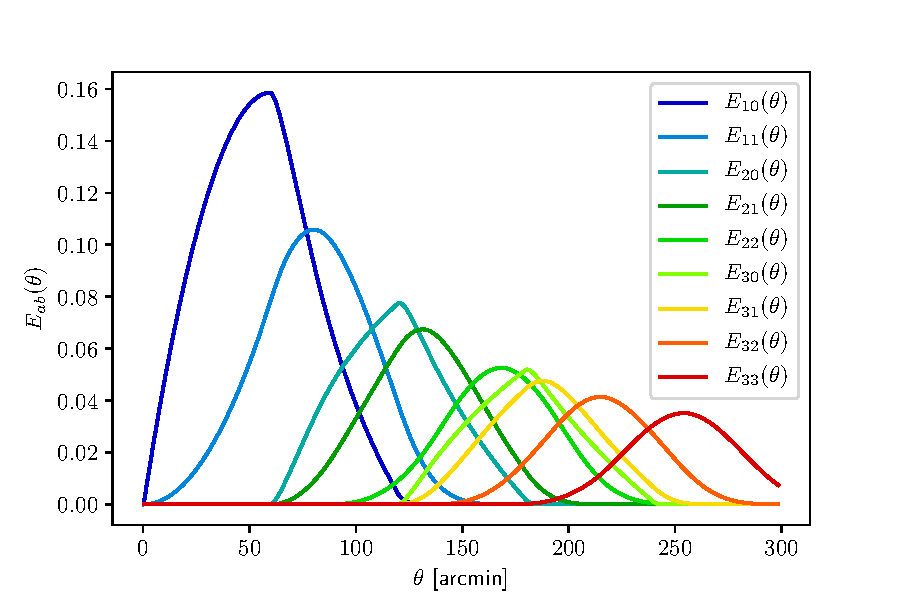
\includegraphics[width = 0.8\textwidth]{eab.pdf}
\caption{The functions $E_{ab}(\theta)$ for the first few possible combinations.}
\label{fig:eab}
\end{figure}
Naturally, to calculate those functions for all possible combinations would be rather tedious, however they are simple to determine numerically (compare Figure \ref{fig:eoftheta_sim}). A plot of these functions can be found in Figure \ref{fig:eab}.

When we now simulate random distributions of the depth-function for a $100\,\rm{deg}^2$-field, a $450\,\rm{deg}^2$-field and a $1000\,\rm{deg}^2$-field, we can compare how they differ from each other and estimate how important finite-field effects are. As can be seen from Figures \ref{fig:100degsqr}, \ref{fig:450degsqr} and \ref{fig:1000degsqr}, the effect is quite significant for a $100\,\rm{deg}^2$-field, but almost negligible for a $1000\,\rm{deg}^2$-field. This leads to the assumption that both for the KiDS- as for the Euclid-survey, finite field effects do not need to be accounted for. However, if the distribution of depth is correlated in the surveys, that might have a noticeable impact on the results.




\chapter{Additional figures and fables}
\section{Additional tables}
\begin{table}[h]
\centering
\caption{Weighted number of galaxies $N$ and average redshift $\la z \ra$ for each percentile of each bin.}
\hspace*{0.5cm}
\begin{tabular}{c|cc|cc|cc|cc|cc}
Percentile & \multicolumn{2}{c|}{Bin 1} & \multicolumn{2}{c|}{Bin 2} & \multicolumn{2}{c|}{Bin 3}& \multicolumn{2}{c|}{Bin 4}& \multicolumn{2}{c}{Bin 5} \\
 & $\la z \ra$ & $N$ & $\la z \ra$ & $N$& $\la z \ra$ & $N$& $\la z \ra$ & $N$& $\la z \ra$ & $N$ \\
\toprule
 1 & 0.36 &  33230 & 0.45 &  45630 & 0.59 &  57873 & 0.78 &  33053 & 0.94 &  23633 \\
 2 & 0.40 &  37848 & 0.48 &  52642 & 0.62 &  69929 & 0.80 &  44464 & 0.97 &  31352 \\
 3 & 0.42 &  38410 & 0.49 &  56986 & 0.64 &  74411 & 0.81 &  47164 & 0.97 &  34352 \\
 4 & 0.44 &  37445 & 0.50 &  54066 & 0.66 &  75132 & 0.82 &  46911 & 0.98 &  34788 \\
 5 & 0.46 &  38698 & 0.52 &  57357 & 0.67 &  75679 & 0.83 &  49620 & 0.99 &  39126 \\
 6 & 0.49 &  40742 & 0.54 &  55456 & 0.69 &  82209 & 0.84 &  53458 & 0.99 &  42326 \\
 7 & 0.51 &  38417 & 0.55 &  56883 & 0.70 &  80228 & 0.85 &  54378 & 1.01 &  44319 \\
 8 & 0.51 &  40110 & 0.56 &  60966 & 0.72 &  91835 & 0.86 &  63515 & 1.01 &  49094 \\
 9 & 0.59 &  39655 & 0.59 &  59207 & 0.75 &  87330 & 0.86 &  59674 & 1.02 &  53566 \\
10 & 0.63 &  41653 & 0.62 &  64526 & 0.80 & 104866 & 0.89 &  79990 & 1.04 &  63426 \\
\bottomrule
\end{tabular}
\label{tab:nvsz}
\end{table}

\clearpage
\section{Results of the MCMC}
\begin{figure}[h]
\centering
	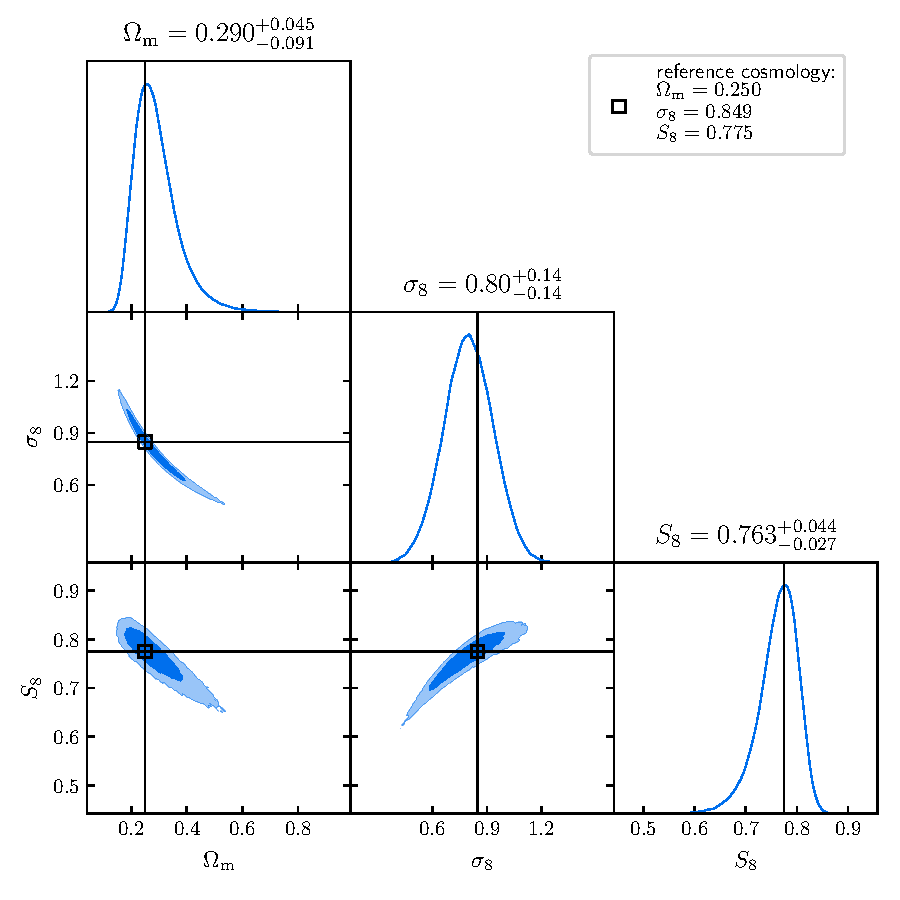
\includegraphics[width=0.7\textwidth]{obscorr.pdf}
	\caption{Bias in the parameters for a KiDS-like Survey.}
	\label{fig:mcmc_kids}
\end{figure}  
\begin{figure}[h]
\centering
	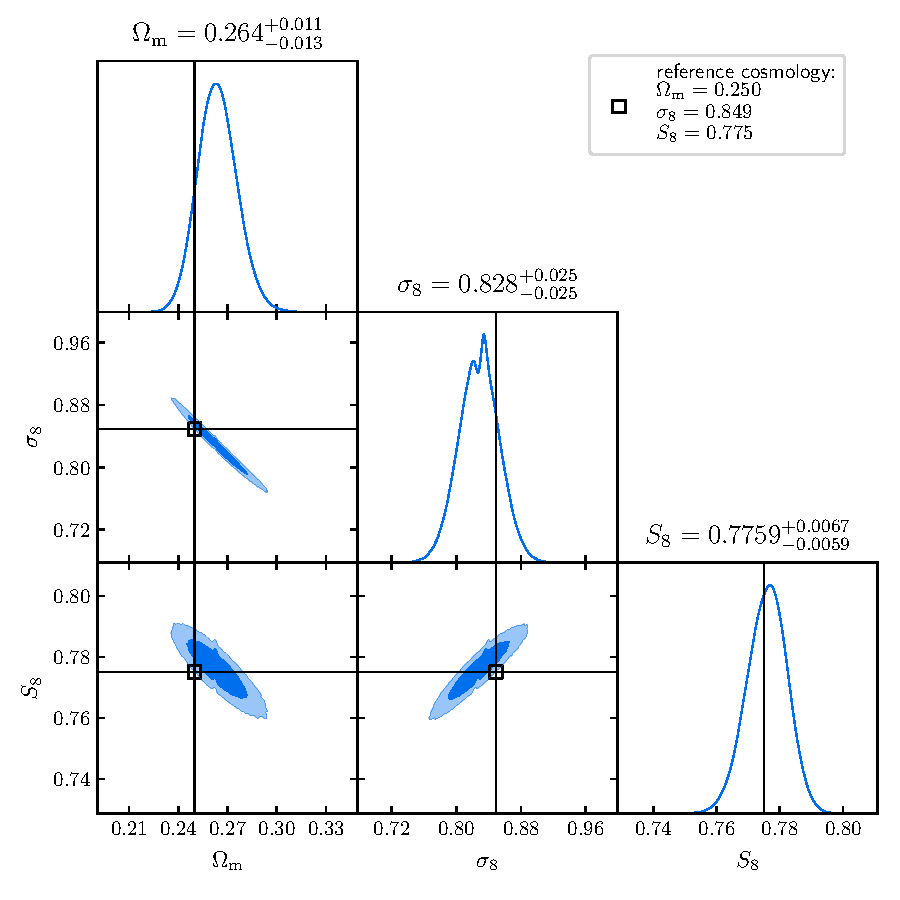
\includegraphics[width=0.7\textwidth]{euclid.pdf}
	\caption{Bias in the parameters for a Euclid-like Survey.}
	\label{fig:mcmc_euclid}
\end{figure}  
\clearpage
\section{Finite field effects}

\begin{figure}[h]
\centering
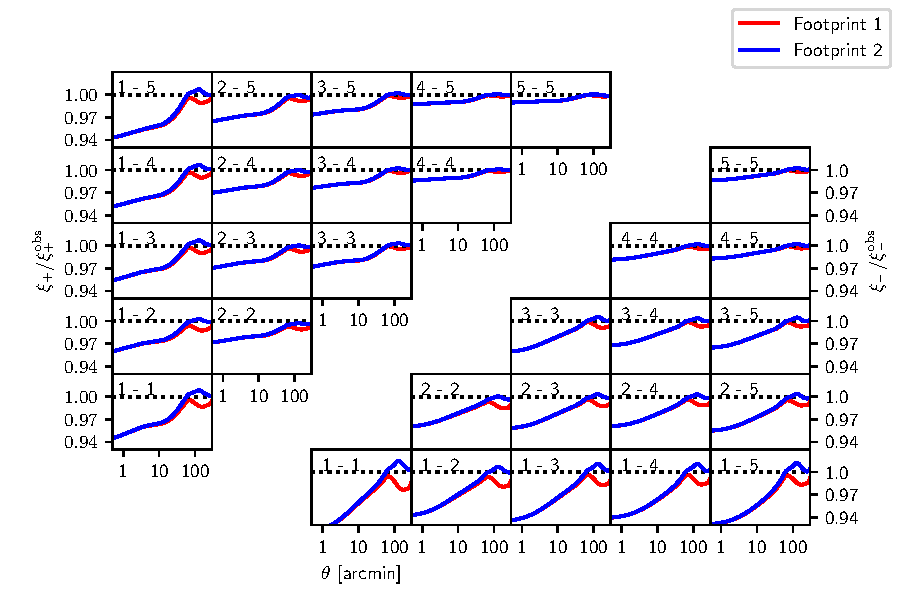
\includegraphics[width=\textwidth]{100degtwofoot_final.pdf}
\caption[Correction of the correlation functions for a $100\,\rm{deg}^2$-field.] {Correction of the correlation functions for two different distributions of percentiles for a $100\,\rm{deg}^2$-field.}
\label{fig:100degsqr}
\end{figure}

\begin{figure}[h]
\centering
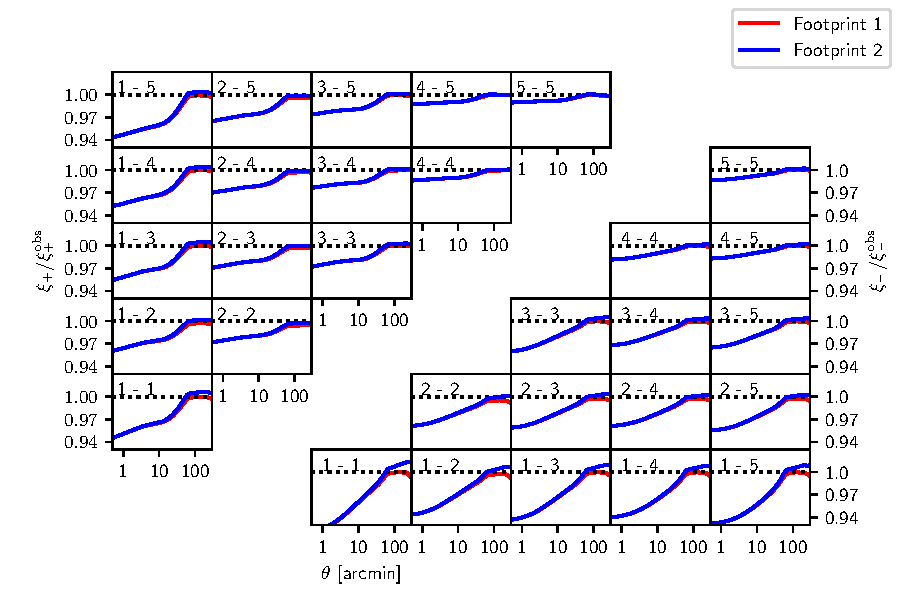
\includegraphics[width=\textwidth]{450degtwofoot_final.pdf}
\caption[Correction of the correlation functions for a $450\,\rm{deg}^2$-field.] {Correction of the correlation functions for two different distributions of percentiles for a $450\,\rm{deg}^2$-field.}
\label{fig:450degsqr}
\end{figure}

\begin{figure}[h]
\centering
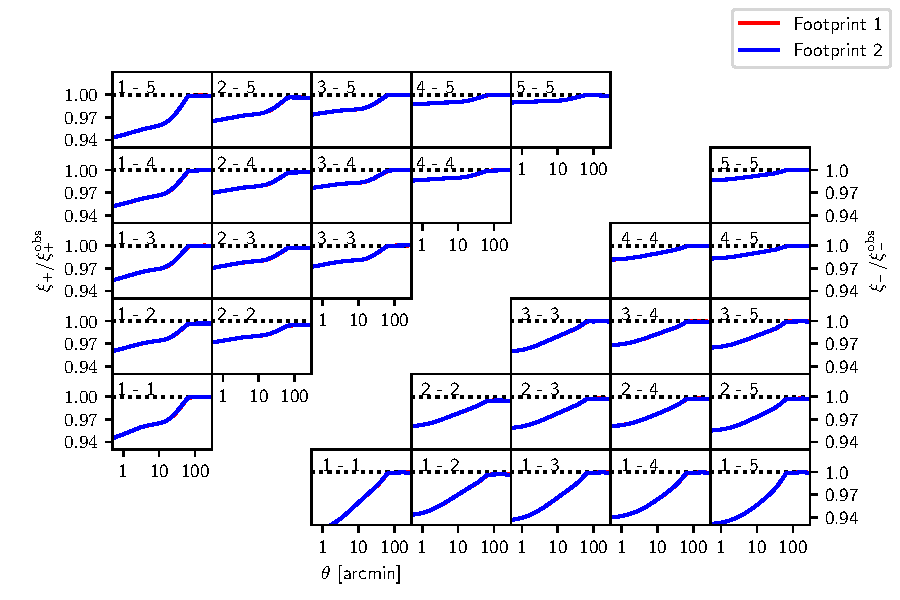
\includegraphics[width=\textwidth]{1000degtwofoot_final.pdf}
\caption[Correction of the correlation functions for a $1000\,\rm{deg}^2$-field.] {Correction of the correlation functions for two different distributions of percentiles for a $1000\,\rm{deg}^2$-field.}
\label{fig:1000degsqr}
\end{figure}

%%% Local Variables: 
%%% mode: latex
%%% TeX-master: "../mythesis"
%%% End: 
